\subsection{Introduction}

\begin{frame}{Acoustic Echo Retrieval}

    % Given the echo model
    % \begin{equation*}
    %     H_{ij}(f) = \sum_{r=0}^{R} \alpha e^{2\pi},
    % \end{equation*}
    % \vfill

    \begin{columns}[T,onlytextwidth]

        \column{0.55\textwidth}
        \begin{alertblock}{The acoustic echoes retrieval (AER) problem}

            \vspace{.1em}
            Estimating early (strong) acoustic reflections:
            \begin{itemize}
                \item their time of arrivals $\rightarrow$ TOAs Estimation
                \\$\hookrightarrow$ sufficient sometimes
                \item their amplitude
                \\$\hookrightarrow$ closed-form form TOA
            \end{itemize}
        \end{alertblock}

        \column{0.4\textwidth}
            \begin{figure}
                \centering
                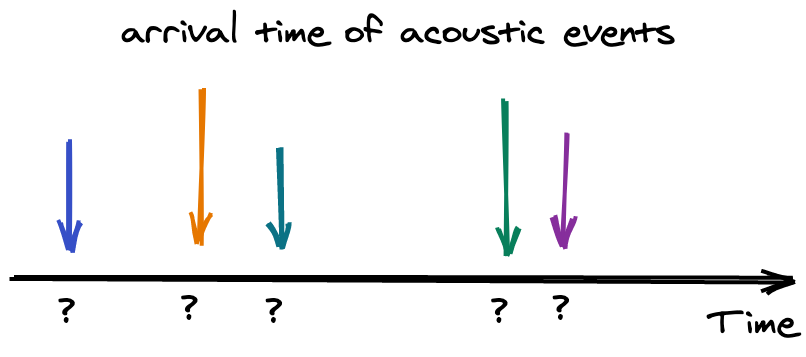
\includegraphics[width=\textwidth]{./figures/arrivals.png}
            \end{figure}

    \end{columns}

    \vfill
    Approaches
    \begin{columns}[T,onlytextwidth]
        \column{0.48\textwidth}
        \centering
        Source signal is
        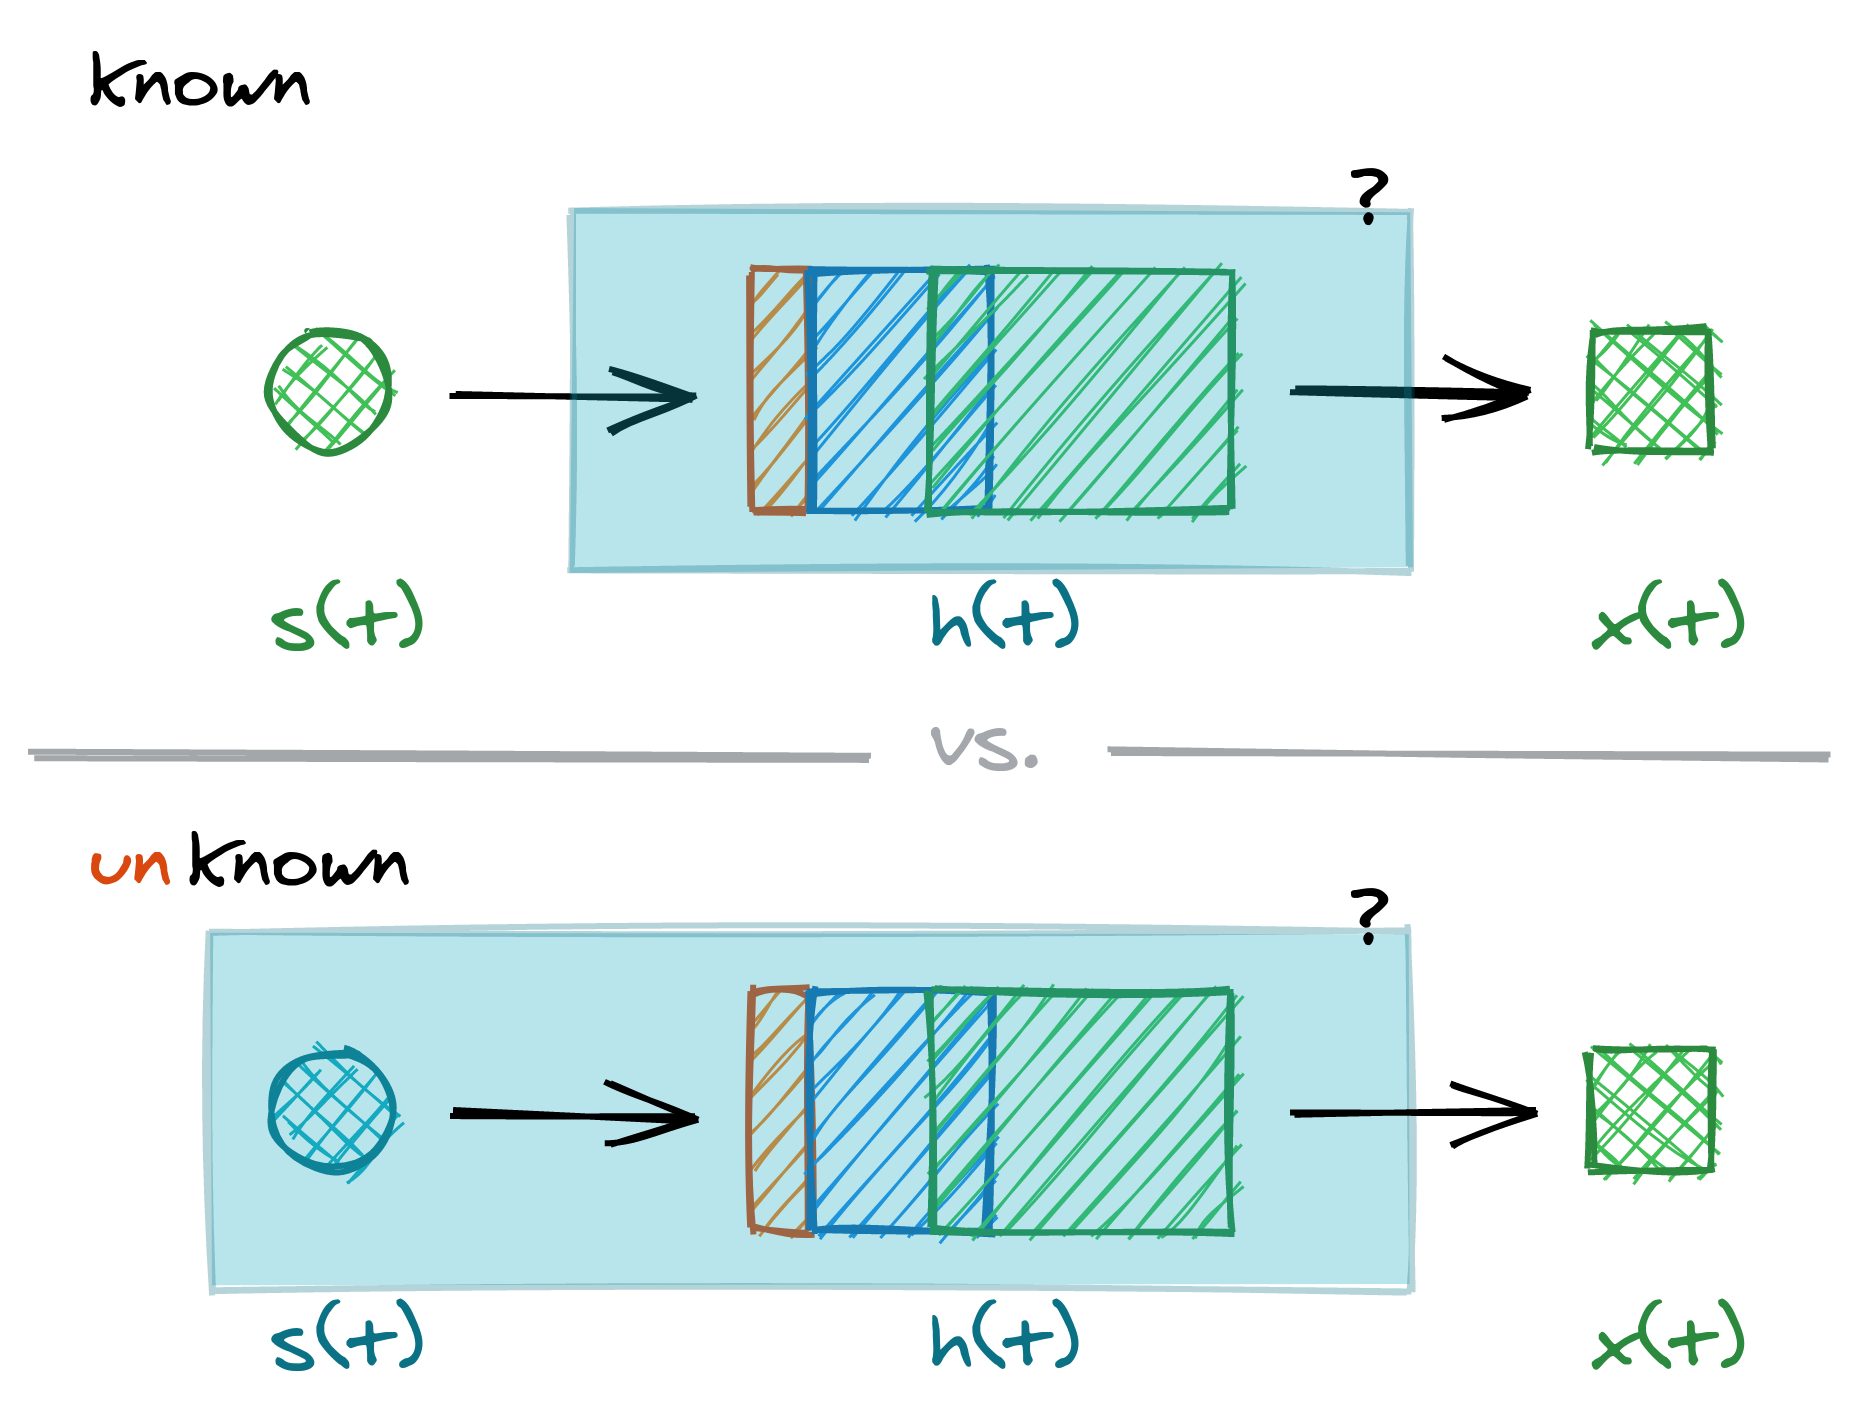
\includegraphics[width=.9\textwidth]{./figures/active-passive.png}
        \hfill

        \only<1>{
            \column{0.48\textwidth}
            \begin{block}{Active approaches}
                \begin{itemize}
                    \item solve and easier problem
                    \item Intrusive or specific setup
                    \item Single microphones
                \end{itemize}
                \textcolor{gray}{\textbf{Application} Sonar, Calibration, Measurements}
            \end{block}
            \begin{block}{Passive approaches}
                \begin{itemize}
                    \item more difficult problem --- blind inverse problem
                    \item Non Intrusive, passive hearing
                    \item Need multi-microphones
                \end{itemize}
                \textcolor{gray}{\textbf{Application} Smart speakers, robot}
            \end{block}
        }
        \only<2>{
            \column{0.48\textwidth}
            \centering
            Estimation is
            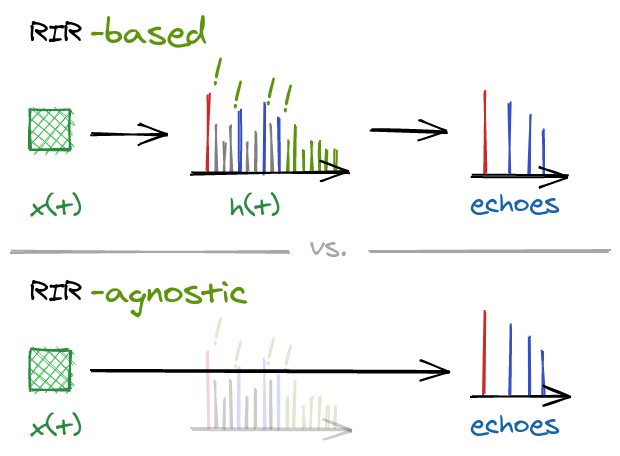
\includegraphics[width=.9\textwidth]{./figures/based-agnostic.png}
        }
    \end{columns}

    \vfill
    \textcolor{myred}{\textbf{Scenario:} signal source, only TOAs and passive system}

\end{frame}

\begin{frame}{Passive Acoustic Echo Estimation}

    \begin{block}{\alert{Passive} Acoustic Echo Estimation:}

        \vspace{1em}
        \small
        \begin{columns}[T,onlytextwidth] % align columns
            \begin{column}{.48\textwidth}
                \textbf{RIR-\alert{based} approaches}
                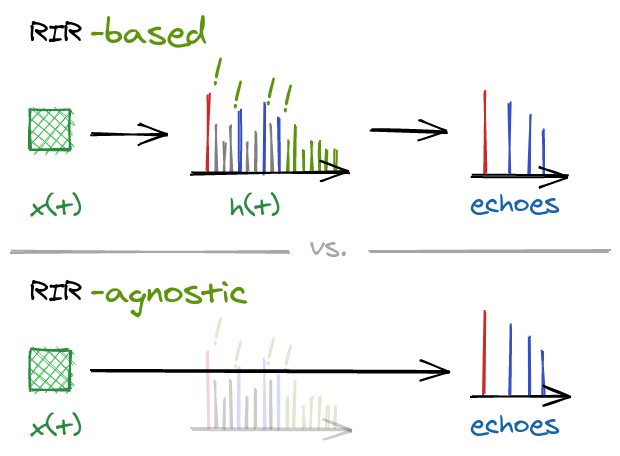
\includegraphics[trim={0 31em 0 7em},clip,width=.9\textwidth]{./figures/based-agnostic.png}
                \begin{enumerate}
                    \item SIMO BCE problem $\implies$ RIRs
                    \item Peak picking and \textit{disambiguation} $\implies$ Echoes
                \end{enumerate}
                Pros
                \begin{itemize}
                    \item SIMO BCE is well studied (elegant framework)
                    \item It works well is some scenarios and in practice
                    \\$\hookrightarrow$ if not limitation
                \end{itemize}
                Cons
                \begin{itemize}
                    \item Full RIR
                    \item dependent of manually tuned peak picking
                    \item Pathological issue (sampling and body-guard
                    \item Complexity
                    \item Non-negativity and sparsity not true
                \end{itemize}
            \end{column}%
            \hfill%
            \begin{column}{.48\textwidth}
                \textbf{RIR-\alert{agnostic} approaches}
                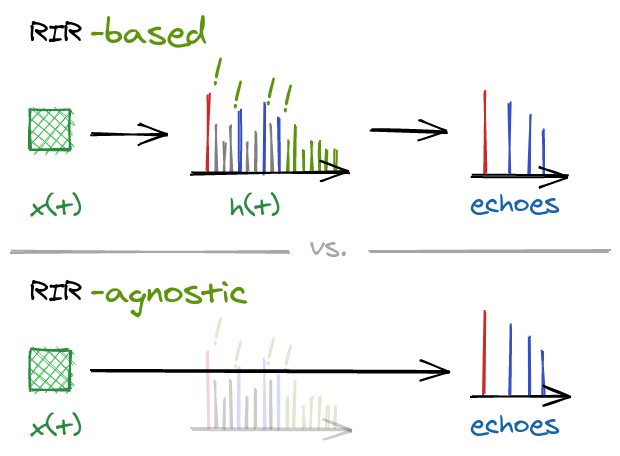
\includegraphics[trim={0 0 0 47em},clip,width=.9\textwidth]{./figures/based-agnostic.png}
                \begin{enumerate}
                    \item Estimation directly in the echoes parameters space $\{\tau,\alpha\}$
                    \\and direction of arrivals can be used instead
                \end{enumerate}
                Performed with
                \begin{itemize}
                    \item Cross-correlation
                    \\on-grid, eg. EM, Acoustic Cameras
                    \item Cross-relation with super-resolution
                    \\off-grid,~\cite{mulan,blaster}
                \end{itemize}
                Pro
                \begin{itemize}
                    \item No need for full RIRs
                    \item Sub-sampling accuracy
                    \item Low complexity
                    \item Sparsity and Non-negativity are respected
                \end{itemize}
                Cons
                \begin{itemize}
                    \item Exploratory
                \end{itemize}
            \end{column}%
        \end{columns}

    \end{block}

\end{frame}

\begin{frame}{AER as discrete SIMO BCE}

    \begin{block}{Key ingredient -- \textit{Cross relation identity}}
        \begin{columns}[onlytextwidth]
        \column{0.6\textwidth}
            \[
                x_i = h_i \ast s
            \]
            \[
                h_2 \ast x_1 = \textcolor{gray}{h_2 \ast h_1 \ast s  = h_1 \ast h_2 \ast s} = h_1 \ast x_2
            \]

            \column{0.3\textwidth}
            \only<1>{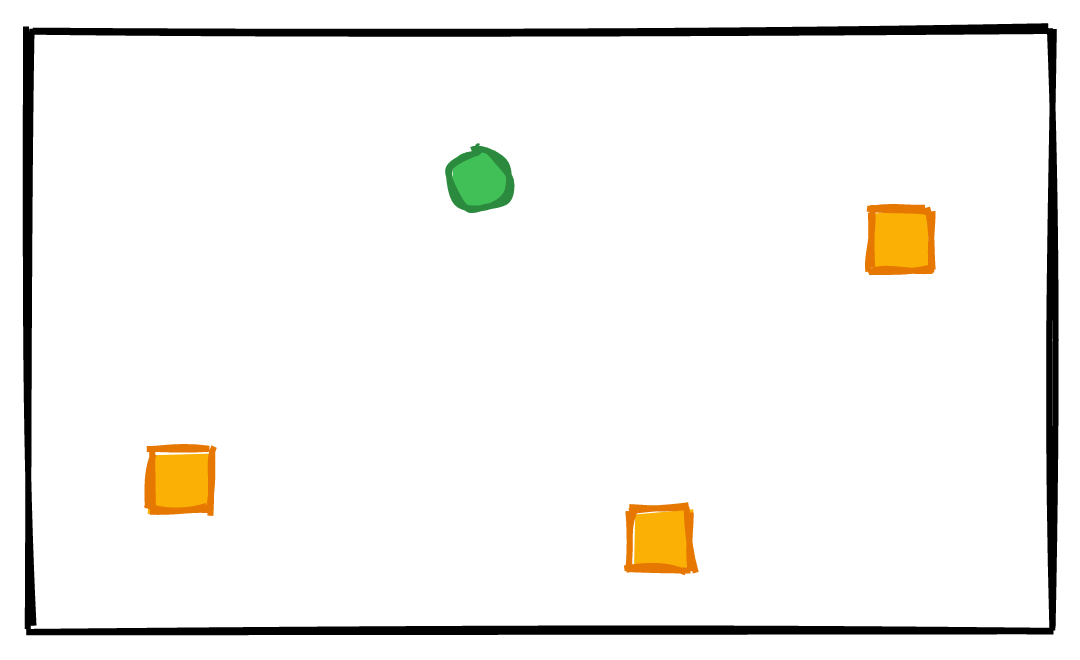
\includegraphics[width=0.9\textwidth]{figures/xrelation1.png}}
            \only<2>{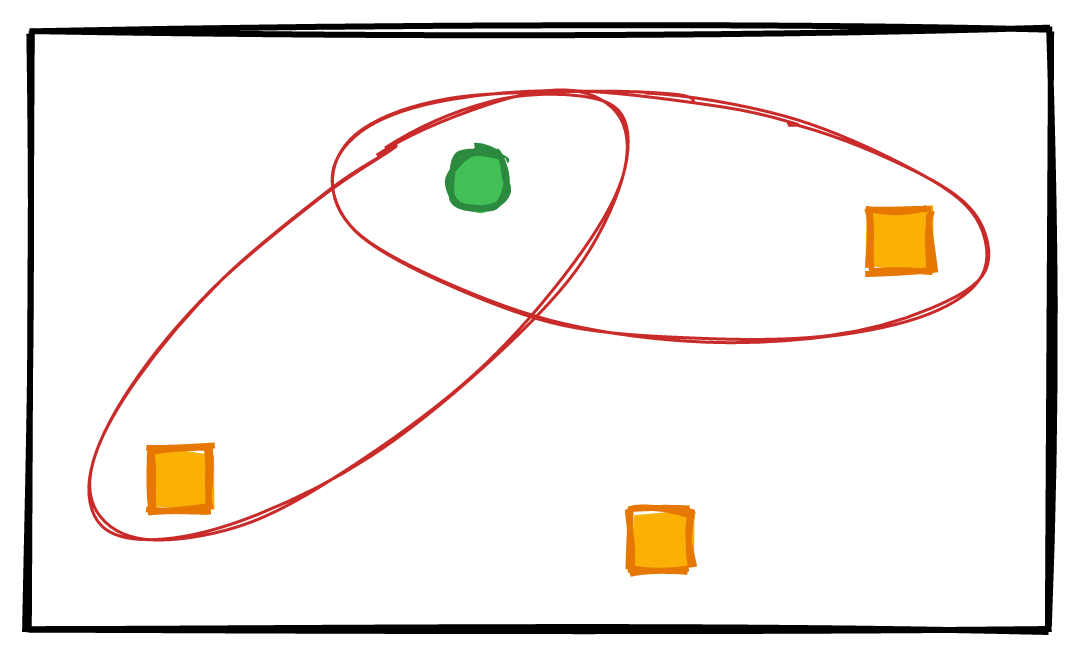
\includegraphics[width=0.9\textwidth]{figures/xrelation2.png}}
        \end{columns}
    \end{block}

    \vspace*{-1em}

    \begin{block}{Ideas:}
    \begin{enumerate}
        \item Sampled version of $x_1,x_2$ are available ($\mathbf{x}_1, \mathbf{x_2}$)
        \item echoes' TOAs $\propto$ sampling frequency
        \item Find echoes $\rightarrow$ \textbf{find sparse vectors} $\mathbf{h}_1, \mathbf{h}_2$ of length $L$
        \item Modeled as \textbf{Lasso}-like problem

        \vspace*{.25em}

        \definecolor{darkblue}{HTML}{154360}
        \definecolor{bluegreen}{HTML}{228BE6}
        \setbeamercolor{postit}{fg=black,bg=bluegreen!10}
        \begin{beamercolorbox}[sep=.5em]{postit}
            \begin{equation*}
                \widehat{\mathbf{h}}_1, \widehat{\mathbf{h}}_2 \in
                \underset{\mathbf{h}_1, \mathbf{h}_2\in\kR^n}{\arg\min}\;
                \Vert \mathbf{x}_1 \tikzmark{a}\ast \mathbf{h}_2 - \mathbf{x}_2 \ast \mathbf{h}_1 \Vert_2^2
                + \lambda \mathcal{P}(\mathbf{h}_1, \mathbf{h}_2)
                \quad\text{s.t.}\quad\mathcal{C}(\mathbf{h}_1, \mathbf{h}_2)
            \end{equation*}
            \vspace{0.5em}
            \hfill {\footnotesize $\mathcal{P}(\mathbf{h}_1, \mathbf{h}_2)$ $\longrightarrow$ sparse promoting regularizer}
            \hfill {\footnotesize $\mathcal{C}(\mathbf{h}_1, \mathbf{h}_2)$ $\longrightarrow$ non-negativity constraints}
        \end{beamercolorbox}

            % \column{0.3\textwidth}
            % \centering
            % \resizebox{\linewidth}{!}{
            %     

\tikzset{every picture/.style={line width=0.75pt}} %set default line width to 0.75pt

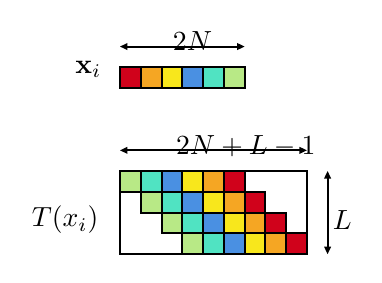
\begin{tikzpicture}[x=0.75pt,y=0.75pt,yscale=-1,xscale=1]
%uncomment if require: \path (0,300); %set diagram left start at 0, and has height of 300

%Shape: Rectangle [id:dp9681290386895156]
\draw   (190,80) -- (280,80) -- (280,120) -- (190,120) -- cycle ;
%Shape: Rectangle [id:dp4105274901835]
\draw  [fill={rgb, 255:red, 208; green, 2; blue, 27 }  ,fill opacity=1 ] (190,30) -- (200,30) -- (200,40) -- (190,40) -- cycle ;
%Shape: Rectangle [id:dp07108913371302106]
\draw  [fill={rgb, 255:red, 245; green, 166; blue, 35 }  ,fill opacity=1 ] (200,30) -- (210,30) -- (210,40) -- (200,40) -- cycle ;
%Shape: Rectangle [id:dp27992457661326675]
\draw  [fill={rgb, 255:red, 248; green, 231; blue, 28 }  ,fill opacity=1 ] (210,30) -- (220,30) -- (220,40) -- (210,40) -- cycle ;
%Shape: Rectangle [id:dp22621399339540804]
\draw  [fill={rgb, 255:red, 74; green, 144; blue, 226 }  ,fill opacity=1 ] (220,30) -- (230,30) -- (230,40) -- (220,40) -- cycle ;
%Shape: Rectangle [id:dp8143232980428775]
\draw  [fill={rgb, 255:red, 80; green, 227; blue, 194 }  ,fill opacity=1 ] (230,30) -- (240,30) -- (240,40) -- (230,40) -- cycle ;
%Shape: Rectangle [id:dp3194122969586535]
\draw  [fill={rgb, 255:red, 184; green, 233; blue, 134 }  ,fill opacity=1 ] (240,30) -- (250,30) -- (250,40) -- (240,40) -- cycle ;
%Straight Lines [id:da5684493017647214]
\draw    (193,20) -- (247,20) ;
\draw [shift={(250,20)}, rotate = 180] [fill={rgb, 255:red, 0; green, 0; blue, 0 }  ][line width=0.08]  [draw opacity=0] (3.57,-1.72) -- (0,0) -- (3.57,1.72) -- cycle    ;
\draw [shift={(190,20)}, rotate = 0] [fill={rgb, 255:red, 0; green, 0; blue, 0 }  ][line width=0.08]  [draw opacity=0] (3.57,-1.72) -- (0,0) -- (3.57,1.72) -- cycle    ;
%Straight Lines [id:da9066793447166841]
\draw    (290,83) -- (290,117) ;
\draw [shift={(290,120)}, rotate = 270] [fill={rgb, 255:red, 0; green, 0; blue, 0 }  ][line width=0.08]  [draw opacity=0] (3.57,-1.72) -- (0,0) -- (3.57,1.72) -- cycle    ;
\draw [shift={(290,80)}, rotate = 90] [fill={rgb, 255:red, 0; green, 0; blue, 0 }  ][line width=0.08]  [draw opacity=0] (3.57,-1.72) -- (0,0) -- (3.57,1.72) -- cycle    ;
%Shape: Rectangle [id:dp8376347441359862]
\draw  [fill={rgb, 255:red, 208; green, 2; blue, 27 }  ,fill opacity=1 ] (250,90) -- (240,90) -- (240,80) -- (250,80) -- cycle ;
%Shape: Rectangle [id:dp7117636003093408]
\draw  [fill={rgb, 255:red, 245; green, 166; blue, 35 }  ,fill opacity=1 ] (240,90) -- (230,90) -- (230,80) -- (240,80) -- cycle ;
%Shape: Rectangle [id:dp4138379160748573]
\draw  [fill={rgb, 255:red, 248; green, 231; blue, 28 }  ,fill opacity=1 ] (230,90) -- (220,90) -- (220,80) -- (230,80) -- cycle ;
%Shape: Rectangle [id:dp3999938091654833]
\draw  [fill={rgb, 255:red, 74; green, 144; blue, 226 }  ,fill opacity=1 ] (220,90) -- (210,90) -- (210,80) -- (220,80) -- cycle ;
%Shape: Rectangle [id:dp9277683628608865]
\draw  [fill={rgb, 255:red, 80; green, 227; blue, 194 }  ,fill opacity=1 ] (210,90) -- (200,90) -- (200,80) -- (210,80) -- cycle ;
%Shape: Rectangle [id:dp38590620029972567]
\draw  [fill={rgb, 255:red, 184; green, 233; blue, 134 }  ,fill opacity=1 ] (200,90) -- (190,90) -- (190,80) -- (200,80) -- cycle ;

%Straight Lines [id:da7133925241736656]
\draw    (193,70) -- (277,70) ;
\draw [shift={(280,70)}, rotate = 180] [fill={rgb, 255:red, 0; green, 0; blue, 0 }  ][line width=0.08]  [draw opacity=0] (3.57,-1.72) -- (0,0) -- (3.57,1.72) -- cycle    ;
\draw [shift={(190,70)}, rotate = 0] [fill={rgb, 255:red, 0; green, 0; blue, 0 }  ][line width=0.08]  [draw opacity=0] (3.57,-1.72) -- (0,0) -- (3.57,1.72) -- cycle    ;
%Shape: Rectangle [id:dp49856978345829306]
\draw  [fill={rgb, 255:red, 208; green, 2; blue, 27 }  ,fill opacity=1 ] (260,100) -- (250,100) -- (250,90) -- (260,90) -- cycle ;
%Shape: Rectangle [id:dp3235825725633823]
\draw  [fill={rgb, 255:red, 245; green, 166; blue, 35 }  ,fill opacity=1 ] (250,100) -- (240,100) -- (240,90) -- (250,90) -- cycle ;
%Shape: Rectangle [id:dp31123598821243614]
\draw  [fill={rgb, 255:red, 248; green, 231; blue, 28 }  ,fill opacity=1 ] (240,100) -- (230,100) -- (230,90) -- (240,90) -- cycle ;
%Shape: Rectangle [id:dp11900662558381525]
\draw  [fill={rgb, 255:red, 74; green, 144; blue, 226 }  ,fill opacity=1 ] (230,100) -- (220,100) -- (220,90) -- (230,90) -- cycle ;
%Shape: Rectangle [id:dp5949312347675072]
\draw  [fill={rgb, 255:red, 80; green, 227; blue, 194 }  ,fill opacity=1 ] (220,100) -- (210,100) -- (210,90) -- (220,90) -- cycle ;
%Shape: Rectangle [id:dp4169331213844353]
\draw  [fill={rgb, 255:red, 184; green, 233; blue, 134 }  ,fill opacity=1 ] (210,100) -- (200,100) -- (200,90) -- (210,90) -- cycle ;

%Shape: Rectangle [id:dp6629627557025272]
\draw  [fill={rgb, 255:red, 208; green, 2; blue, 27 }  ,fill opacity=1 ] (270,110) -- (260,110) -- (260,100) -- (270,100) -- cycle ;
%Shape: Rectangle [id:dp31604732616257436]
\draw  [fill={rgb, 255:red, 245; green, 166; blue, 35 }  ,fill opacity=1 ] (260,110) -- (250,110) -- (250,100) -- (260,100) -- cycle ;
%Shape: Rectangle [id:dp09107227856524347]
\draw  [fill={rgb, 255:red, 248; green, 231; blue, 28 }  ,fill opacity=1 ] (250,110) -- (240,110) -- (240,100) -- (250,100) -- cycle ;
%Shape: Rectangle [id:dp7267681930473228]
\draw  [fill={rgb, 255:red, 74; green, 144; blue, 226 }  ,fill opacity=1 ] (240,110) -- (230,110) -- (230,100) -- (240,100) -- cycle ;
%Shape: Rectangle [id:dp29680219911700556]
\draw  [fill={rgb, 255:red, 80; green, 227; blue, 194 }  ,fill opacity=1 ] (230,110) -- (220,110) -- (220,100) -- (230,100) -- cycle ;
%Shape: Rectangle [id:dp12926304976478886]
\draw  [fill={rgb, 255:red, 184; green, 233; blue, 134 }  ,fill opacity=1 ] (220,110) -- (210,110) -- (210,100) -- (220,100) -- cycle ;

%Shape: Rectangle [id:dp11163148873105677]
\draw  [fill={rgb, 255:red, 208; green, 2; blue, 27 }  ,fill opacity=1 ] (280,120) -- (270,120) -- (270,110) -- (280,110) -- cycle ;
%Shape: Rectangle [id:dp3773220154233181]
\draw  [fill={rgb, 255:red, 245; green, 166; blue, 35 }  ,fill opacity=1 ] (270,120) -- (260,120) -- (260,110) -- (270,110) -- cycle ;
%Shape: Rectangle [id:dp21547184217790727]
\draw  [fill={rgb, 255:red, 248; green, 231; blue, 28 }  ,fill opacity=1 ] (260,120) -- (250,120) -- (250,110) -- (260,110) -- cycle ;
%Shape: Rectangle [id:dp30710052799291054]
\draw  [fill={rgb, 255:red, 74; green, 144; blue, 226 }  ,fill opacity=1 ] (250,120) -- (240,120) -- (240,110) -- (250,110) -- cycle ;
%Shape: Rectangle [id:dp8950222427502034]
\draw  [fill={rgb, 255:red, 80; green, 227; blue, 194 }  ,fill opacity=1 ] (240,120) -- (230,120) -- (230,110) -- (240,110) -- cycle ;
%Shape: Rectangle [id:dp01705103269779118]
\draw  [fill={rgb, 255:red, 184; green, 233; blue, 134 }  ,fill opacity=1 ] (230,120) -- (220,120) -- (220,110) -- (230,110) -- cycle ;


% Text Node
\draw (167,25.4) node [anchor=north west][inner sep=0.75pt] {$\mathbf{x}_{i}$};
% Text Node
\draw (146,95.4) node [anchor=north west][inner sep=0.75pt] {$\mathscr{T}( x_{i})$};
% Text Node
\draw (214,11.4) node [anchor=north west][inner sep=0.75pt] {$2N$};
% Text Node
\draw (291,97.4) node [anchor=north west][inner sep=0.75pt] {$L$};
% Text Node
\draw (215.5,61.4) node [anchor=north west][inner sep=0.75pt] {$2N+L-1$};


\end{tikzpicture}

            % }
    \end{enumerate}
    \textcolor{gray}{\small $\mathbf{x_i} \ast \mathbf{h}_j$ computed as $\mathcal{T}(\mathbf{x}_i) \mathbf{h_j} \in \mathcal{O}(L^2)$}

    \vfill
    \begin{center}
        \definecolor{mygreen}{RGB}{30,132,73}
        \textcolor{mygreen}{$\checkmark$}  \cite{Lin2007} \qquad \textcolor{mygreen}{$\checkmark$} \cite{Aissa-El-Bey2008} \\
        \textcolor{mygreen}{$\checkmark$} \cite{Kowalczyk2013} \qquad \textcolor{mygreen}{$\checkmark$} \cite{Crocco2015}
    \end{center}

    \end{block}

    % \begin{tikzpicture}[overlay,remember picture,x=1mm,y=-1mm,shift={(current page.north west)}]
    %     \node  (mypic) at (100,80) {\resizebox{35mm}{!}{

\tikzset{every picture/.style={line width=0.75pt}} %set default line width to 0.75pt

\begin{tikzpicture}[x=0.75pt,y=0.75pt,yscale=-1,xscale=1]
%uncomment if require: \path (0,300); %set diagram left start at 0, and has height of 300

%Shape: Rectangle [id:dp9681290386895156]
\draw   (190,80) -- (280,80) -- (280,120) -- (190,120) -- cycle ;
%Shape: Rectangle [id:dp4105274901835]
\draw  [fill={rgb, 255:red, 208; green, 2; blue, 27 }  ,fill opacity=1 ] (190,30) -- (200,30) -- (200,40) -- (190,40) -- cycle ;
%Shape: Rectangle [id:dp07108913371302106]
\draw  [fill={rgb, 255:red, 245; green, 166; blue, 35 }  ,fill opacity=1 ] (200,30) -- (210,30) -- (210,40) -- (200,40) -- cycle ;
%Shape: Rectangle [id:dp27992457661326675]
\draw  [fill={rgb, 255:red, 248; green, 231; blue, 28 }  ,fill opacity=1 ] (210,30) -- (220,30) -- (220,40) -- (210,40) -- cycle ;
%Shape: Rectangle [id:dp22621399339540804]
\draw  [fill={rgb, 255:red, 74; green, 144; blue, 226 }  ,fill opacity=1 ] (220,30) -- (230,30) -- (230,40) -- (220,40) -- cycle ;
%Shape: Rectangle [id:dp8143232980428775]
\draw  [fill={rgb, 255:red, 80; green, 227; blue, 194 }  ,fill opacity=1 ] (230,30) -- (240,30) -- (240,40) -- (230,40) -- cycle ;
%Shape: Rectangle [id:dp3194122969586535]
\draw  [fill={rgb, 255:red, 184; green, 233; blue, 134 }  ,fill opacity=1 ] (240,30) -- (250,30) -- (250,40) -- (240,40) -- cycle ;
%Straight Lines [id:da5684493017647214]
\draw    (193,20) -- (247,20) ;
\draw [shift={(250,20)}, rotate = 180] [fill={rgb, 255:red, 0; green, 0; blue, 0 }  ][line width=0.08]  [draw opacity=0] (3.57,-1.72) -- (0,0) -- (3.57,1.72) -- cycle    ;
\draw [shift={(190,20)}, rotate = 0] [fill={rgb, 255:red, 0; green, 0; blue, 0 }  ][line width=0.08]  [draw opacity=0] (3.57,-1.72) -- (0,0) -- (3.57,1.72) -- cycle    ;
%Straight Lines [id:da9066793447166841]
\draw    (290,83) -- (290,117) ;
\draw [shift={(290,120)}, rotate = 270] [fill={rgb, 255:red, 0; green, 0; blue, 0 }  ][line width=0.08]  [draw opacity=0] (3.57,-1.72) -- (0,0) -- (3.57,1.72) -- cycle    ;
\draw [shift={(290,80)}, rotate = 90] [fill={rgb, 255:red, 0; green, 0; blue, 0 }  ][line width=0.08]  [draw opacity=0] (3.57,-1.72) -- (0,0) -- (3.57,1.72) -- cycle    ;
%Shape: Rectangle [id:dp8376347441359862]
\draw  [fill={rgb, 255:red, 208; green, 2; blue, 27 }  ,fill opacity=1 ] (250,90) -- (240,90) -- (240,80) -- (250,80) -- cycle ;
%Shape: Rectangle [id:dp7117636003093408]
\draw  [fill={rgb, 255:red, 245; green, 166; blue, 35 }  ,fill opacity=1 ] (240,90) -- (230,90) -- (230,80) -- (240,80) -- cycle ;
%Shape: Rectangle [id:dp4138379160748573]
\draw  [fill={rgb, 255:red, 248; green, 231; blue, 28 }  ,fill opacity=1 ] (230,90) -- (220,90) -- (220,80) -- (230,80) -- cycle ;
%Shape: Rectangle [id:dp3999938091654833]
\draw  [fill={rgb, 255:red, 74; green, 144; blue, 226 }  ,fill opacity=1 ] (220,90) -- (210,90) -- (210,80) -- (220,80) -- cycle ;
%Shape: Rectangle [id:dp9277683628608865]
\draw  [fill={rgb, 255:red, 80; green, 227; blue, 194 }  ,fill opacity=1 ] (210,90) -- (200,90) -- (200,80) -- (210,80) -- cycle ;
%Shape: Rectangle [id:dp38590620029972567]
\draw  [fill={rgb, 255:red, 184; green, 233; blue, 134 }  ,fill opacity=1 ] (200,90) -- (190,90) -- (190,80) -- (200,80) -- cycle ;

%Straight Lines [id:da7133925241736656]
\draw    (193,70) -- (277,70) ;
\draw [shift={(280,70)}, rotate = 180] [fill={rgb, 255:red, 0; green, 0; blue, 0 }  ][line width=0.08]  [draw opacity=0] (3.57,-1.72) -- (0,0) -- (3.57,1.72) -- cycle    ;
\draw [shift={(190,70)}, rotate = 0] [fill={rgb, 255:red, 0; green, 0; blue, 0 }  ][line width=0.08]  [draw opacity=0] (3.57,-1.72) -- (0,0) -- (3.57,1.72) -- cycle    ;
%Shape: Rectangle [id:dp49856978345829306]
\draw  [fill={rgb, 255:red, 208; green, 2; blue, 27 }  ,fill opacity=1 ] (260,100) -- (250,100) -- (250,90) -- (260,90) -- cycle ;
%Shape: Rectangle [id:dp3235825725633823]
\draw  [fill={rgb, 255:red, 245; green, 166; blue, 35 }  ,fill opacity=1 ] (250,100) -- (240,100) -- (240,90) -- (250,90) -- cycle ;
%Shape: Rectangle [id:dp31123598821243614]
\draw  [fill={rgb, 255:red, 248; green, 231; blue, 28 }  ,fill opacity=1 ] (240,100) -- (230,100) -- (230,90) -- (240,90) -- cycle ;
%Shape: Rectangle [id:dp11900662558381525]
\draw  [fill={rgb, 255:red, 74; green, 144; blue, 226 }  ,fill opacity=1 ] (230,100) -- (220,100) -- (220,90) -- (230,90) -- cycle ;
%Shape: Rectangle [id:dp5949312347675072]
\draw  [fill={rgb, 255:red, 80; green, 227; blue, 194 }  ,fill opacity=1 ] (220,100) -- (210,100) -- (210,90) -- (220,90) -- cycle ;
%Shape: Rectangle [id:dp4169331213844353]
\draw  [fill={rgb, 255:red, 184; green, 233; blue, 134 }  ,fill opacity=1 ] (210,100) -- (200,100) -- (200,90) -- (210,90) -- cycle ;

%Shape: Rectangle [id:dp6629627557025272]
\draw  [fill={rgb, 255:red, 208; green, 2; blue, 27 }  ,fill opacity=1 ] (270,110) -- (260,110) -- (260,100) -- (270,100) -- cycle ;
%Shape: Rectangle [id:dp31604732616257436]
\draw  [fill={rgb, 255:red, 245; green, 166; blue, 35 }  ,fill opacity=1 ] (260,110) -- (250,110) -- (250,100) -- (260,100) -- cycle ;
%Shape: Rectangle [id:dp09107227856524347]
\draw  [fill={rgb, 255:red, 248; green, 231; blue, 28 }  ,fill opacity=1 ] (250,110) -- (240,110) -- (240,100) -- (250,100) -- cycle ;
%Shape: Rectangle [id:dp7267681930473228]
\draw  [fill={rgb, 255:red, 74; green, 144; blue, 226 }  ,fill opacity=1 ] (240,110) -- (230,110) -- (230,100) -- (240,100) -- cycle ;
%Shape: Rectangle [id:dp29680219911700556]
\draw  [fill={rgb, 255:red, 80; green, 227; blue, 194 }  ,fill opacity=1 ] (230,110) -- (220,110) -- (220,100) -- (230,100) -- cycle ;
%Shape: Rectangle [id:dp12926304976478886]
\draw  [fill={rgb, 255:red, 184; green, 233; blue, 134 }  ,fill opacity=1 ] (220,110) -- (210,110) -- (210,100) -- (220,100) -- cycle ;

%Shape: Rectangle [id:dp11163148873105677]
\draw  [fill={rgb, 255:red, 208; green, 2; blue, 27 }  ,fill opacity=1 ] (280,120) -- (270,120) -- (270,110) -- (280,110) -- cycle ;
%Shape: Rectangle [id:dp3773220154233181]
\draw  [fill={rgb, 255:red, 245; green, 166; blue, 35 }  ,fill opacity=1 ] (270,120) -- (260,120) -- (260,110) -- (270,110) -- cycle ;
%Shape: Rectangle [id:dp21547184217790727]
\draw  [fill={rgb, 255:red, 248; green, 231; blue, 28 }  ,fill opacity=1 ] (260,120) -- (250,120) -- (250,110) -- (260,110) -- cycle ;
%Shape: Rectangle [id:dp30710052799291054]
\draw  [fill={rgb, 255:red, 74; green, 144; blue, 226 }  ,fill opacity=1 ] (250,120) -- (240,120) -- (240,110) -- (250,110) -- cycle ;
%Shape: Rectangle [id:dp8950222427502034]
\draw  [fill={rgb, 255:red, 80; green, 227; blue, 194 }  ,fill opacity=1 ] (240,120) -- (230,120) -- (230,110) -- (240,110) -- cycle ;
%Shape: Rectangle [id:dp01705103269779118]
\draw  [fill={rgb, 255:red, 184; green, 233; blue, 134 }  ,fill opacity=1 ] (230,120) -- (220,120) -- (220,110) -- (230,110) -- cycle ;


% Text Node
\draw (167,25.4) node [anchor=north west][inner sep=0.75pt] {$\mathbf{x}_{i}$};
% Text Node
\draw (146,95.4) node [anchor=north west][inner sep=0.75pt] {$\mathscr{T}( x_{i})$};
% Text Node
\draw (214,11.4) node [anchor=north west][inner sep=0.75pt] {$2N$};
% Text Node
\draw (291,97.4) node [anchor=north west][inner sep=0.75pt] {$L$};
% Text Node
\draw (215.5,61.4) node [anchor=north west][inner sep=0.75pt] {$2N+L-1$};


\end{tikzpicture}
}}
    % \end{tikzpicture}

 \end{frame}

\begin{frame}{Limitations \& bottleneck}

    \begin{block}{On-grid estimation}
        \begin{itemize}
        \item Sparsity and non-negativity Echoes are not necessarily ``on grid''

        \item \emph{Body guard} effect \cite{duval2013}

        % Just wrote it for you...
        % I remember that was a point for decrete vs continous
        \begin{itemize}
            \item[$\rightarrow$] low recall $\implies$ low accuracy % (2 echoes instead of 1)
            \item[$\rightarrow$] slow convergence % bouncing between 2 echoes
        \end{itemize}
        \end{itemize}
    \end{block}

    \begin{block}{... and Pick Picking}
        \begin{itemize}
            \item[$\rightarrow$] Manually tuned peaking or peak disambiguation
        \end{itemize}
    \end{block}

    \vfill

    \begin{block}{Increase the sampling frequency, $F_s$}
        \begin{itemize}
            \item[$\rightarrow$] Increase Precision
        \end{itemize}
    \end{block}

    \begin{block}{Computational bottleneck}
    \begin{itemize}

        \item Bigger vectors and matrices
        \begin{itemize}
            \item[$\longrightarrow$] memory usage
        \end{itemize}

        \vspace*{.5em}

        \item Computational complexity: at best $\mathcal{O}(F_s^2)$ per iteration

        \item the higher the sampling frequency, the more ill-conditioned \\
        \begin{itemize}
            \item[$\longrightarrow$] slow convergence
        \end{itemize}
        \end{itemize}

    \end{block}

    \begin{textblock}{5}(10, 3)
        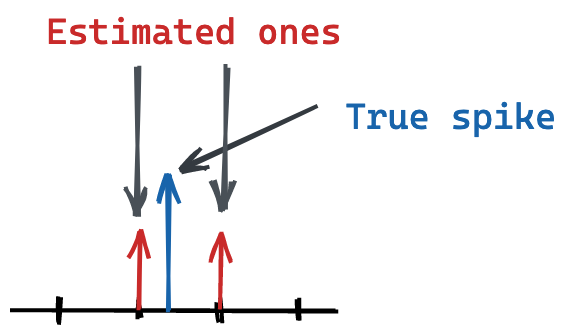
\includegraphics[width=\columnwidth]{figures/bodyguard.png}
    \end{textblock}

\end{frame}

\subsection{\blaster}

\begin{frame}{\blaster - Off-grid BCE}
    \begin{block}{\textbf{Observation 1:} the cross relation remains true in the frequency domain}
        \begin{equation*}
            \mathcal{F}x_1 \cdot \mathcal{F}h_2 (\sfrac{n}{F_s}) = \mathcal{F}x_2 \cdot \mathcal{F}h_1(\sfrac{n}{F_s}) \qquad n=0\dots N-1
        \end{equation*}
        \end{block}

        \vspace{.5em}

        \begin{block}{\textbf{Observation 2:} $\mathcal{F}\delta_{\mathrm{echo}}$ is known in closed-form}
        \end{block}

        \vspace{1.em}

        \begin{block}{\textbf{Observation 3:} $\mathcal{F}{\mathrm{x_i}}$ can be (well) approximated by DFT}
        \begin{equation*}
            \mathbf{X}_i = \texttt{DFT}(\mathbf{x}_i) \simeq  \mathcal{F}{\mathbf{x}_i}(nF_s) \qquad n=0\dots N-1
        \end{equation*}
        \end{block}


    %    \vspace{1.5em}
        \definecolor{darkblue}{HTML}{154360}
        \definecolor{bluegreen}{HTML}{228BE6}
        \setbeamercolor{block title}{fg=white,bg=darkblue}
        \setbeamercolor{block body}{fg=black,bg=bluegreen!10}

        \begin{block}{\textbf{Idea:} Recover echoes by matching a finite number of frequencies}
        \begin{equation*}
            \underset{h_1,h_2 \in \substack{\text{measure} \\ \text{space}}}{\arg\min} \;
            \tfrac{1}{2} \kvvbar{
                \mathbf{X}_1 \cdot \mathcal{F}h_2 (f) - \mathbf{X}_2 \cdot \mathcal{F}h_1(f)
            }_2^2
            + \lambda \kvvbar{h_1 + h_2}_{\mathrm{TV}}
            \quad
            \text{s.t.}\;
            \begin{cases}
                h_1(\{0\})=1 \\
                h_l \geq 0
                \end{cases}
        \end{equation*}
        \end{block}

        \begin{center}
            Instance of a \textbf{BLasso} problem \cite{Bredies2013} (Sliding Frank-Wolfe algorithm)
        \end{center}

        \begin{center}

            \textcolor{mygreen}{\checkmark{no Toeplitz matrix} \qquad \checkmark \, \parbox{8.5em}{Solutions is \\ a train of Dirac} \qquad \checkmark \, \parbox{8em}{anchor prevents \\ trivial solution}}
        \end{center}
\end{frame}

\begin{frame}{\blaster - Experiments}
    \begin{block}{Experiments}
        \begin{itemize}
            \item simulation data with ISM with Pyroomacoustics
            \item 1 source, 2 microphones, random room geometry
            \item Full RIRs
            \item 2 sources: broadband and speech
            \item 2 datasets: different SNR, different RT60
        \end{itemize}
    \end{block}

    \begin{block}{Methods}
        \begin{itemize}
            \item BSN: Blind Sparse and Nonnegative SIMO BCE~\cite{Lin2007}
            \item IL1C: Iteratively-weighted $\ell_1$ Constraint SIME BCE~\cite{Crocco2015}
            \item \blaster: Proposed off-grid approach
        \end{itemize}
    \end{block}

    \begin{block}{Metrics}
        \begin{itemize}
            \item RMSE
            \item Precision
        \end{itemize}
    \end{block}

\end{frame}

\begin{frame}{\blaster - Results}

\end{frame}

\subsection{\lantern}

\begin{frame}{\lantern - data-driven AER}

    \begin{block}{\textbf{Observation 1:} Mapping from observation to echo is extremely difficult}
        Later echoes are not considered, may help
    \end{block}

    \begin{block}{\textbf{Observation 2:} We have acoustic simulators}
        Acoustic simulators based on ISM
        \\source position, room $\leftarrow$ reverberation elements $\leftarrow$
        \\annotation for free
    \end{block}

    \begin{block}{\textbf{Observation 3:} (Deep) Learning-based methods successful for localization}
        Echoes are strongly related to the source position
    \end{block}

    \begin{alertblock}{\textbf{Idea:} Use Deep Learning for AER}
        \begin{itemize}
            \item Extend previous work on source localization for Echo Estimation
            \item Estimate the first echo TOA
            \\$\hookrightarrow$ simple case, but with important application in SSL
        \end{itemize}
    \end{alertblock}

\end{frame}

\begin{frame}{\lantern - Data \& Models}
    \begin{block}{Data}
        \begin{itemize}
            \item train:
            \\$\hookrightarrow$ artificially generated RIR
            \\$\hookrightarrow$ white noise + noise
            \\$\hookrightarrow$ instantaneous RTF
            \item test:
            \\$\hookrightarrow$ artificially generated RIR
            \\$\hookrightarrow$ white noise, speech + noise
            \\$\hookrightarrow$ instantaneous RTF
        \end{itemize}
    \end{block}

    \begin{block}{Architecture}
        \begin{itemize}
            \item models: MLP, CNN
            \item loss: Multi-class regression problem
            \\$\hookrightarrow$ RMSE
            \\$\hookrightarrow$ Gaussian regression + uncertainty
            \\$\hookrightarrow$ Student Regression + uncertainty
        \end{itemize}
    \end{block}

\end{frame}

\begin{frame}{\lantern - Experiments \& Resuls}
    \begin{block}{Experiments}
        \begin{enumerate}
            \item MLP
            \item CNN
            \item CNN + Noise
            \item CNN + Gaussian
            \item CNN + Student
        \end{enumerate}
    \end{block}

    \begin{block}{Results}
        \begin{enumerate}
            \item MLP
            \item CNN
            \item CNN + Noise
            \item CNN + Gaussian
            \item CNN + Student
        \end{enumerate}
    \end{block}

\end{frame}

\subsection{Interim conclusion (2/4)}

\begin{frame}{Interim conclusion (2/4)}
    \begin{block}{on Acoustic Echo Retrieval:}
        \begin{itemize}
            \item Most of the literature is on Passive and RIR-based, with on-grid approaches
            \item On-grid approaches suffers by the off-grid nature of the echoes (complexity, sampling)
        \end{itemize}
    \end{block}

    \begin{block}{on \blaster:}
        \begin{itemize}
            \item[\cmark] off-grid parameter-free which exploit dirac closed-form model (non negativity and sparsity)
            \item[\cmark] smaller RMSE due to super-resolution, better for small \# of echoes
            \item[\xmark] source dependent and on number of echoes
            \item[\xmark] validate only on synthetic data
            \item[$\rightarrow$] Multichannel and RTF-based extention
        \end{itemize}
    \end{block}

    \begin{block}{on \lantern:}
        \begin{itemize}
            \item[\cmark] promising results for first echo estimation
            \item[\cmark] direct application for table top application
            \item[\xmark] difficult extention
            \item[\xmark] need for real data validation
            \item[$\rightarrow$] physically-constrained neural network
            \item[$\rightarrow$] missing frequencies in the input
        \end{itemize}
    \end{block}
\end{frame}